\appendix

\section{Algorithms}\label{app:algorithms}

Algorithm~\ref{alg:naive} is the na\"ive backward proof-search procedure
of Hou~\cite[Algorithm~2, p.~67]{hou2021fundamentals}, rewritten in the
notation used throughout this paper; Algorithm~\ref{alg:priority-id} is
the full priority-ID pseudocode.

% Requires \usepackage{algorithm} and \usepackage{algpseudocode}.
% This fragment is intended to be included from report/report.tex.
\begin{algorithm}
  \caption{Na\"ive backward proof search for LK$'$ (Algorithm~2 of
  \cite[p.~67]{hou2021fundamentals})}\label{alg:naive}
  \begin{algorithmic}[1]
    \Require First-order formula $A$
    \Ensure Derivation tree in LK$'$, or report no proof found
    \State build the bottom sequent $\vdash A$
    \ForAll{top sequents on an open branch}
    \If{any of $\mathit{id}, \top R, \bot L$ is applicable}
    \State apply the rule backwards and close the branch
    \ElsIf{any of $\wedge L, \vee R, {\rightarrow}R, \neg L, \neg R,
    \forall R, \exists L$ is applicable}
    \State apply the rule backwards
    \ElsIf{any of $\wedge R, \vee L, {\rightarrow}L$ is applicable}
    \State apply the rule backwards and create a new branch
    \ElsIf{$\forall L$ or $\exists R$ is applicable, and there is a
      term $t$ that has not been used to instantiate the quantified
    variable $x$ in this formula}
    \State apply the rule backwards, substituting $x$ with $t$
    \ElsIf{$\forall L$ or $\exists R$ is applicable}
    \State apply the rule backwards and create a fresh term
    \Else
    \State stop
    \EndIf
    \EndFor
  \end{algorithmic}
\end{algorithm}


% Requires \usepackage{algorithm} and \usepackage{algpseudocode}.
% This fragment is intended to be included from report/samplepaper.tex.

\begin{algorithm}[t]
  \caption{Priority-ID backward proof search for LK$'$}\label{alg:priority-id}
  \begin{algorithmic}[1]
    \Require Goal sequent $S_0$, maximum depth $D$, maximum steps $N$,
      timeout deadline $T$, fresh-term budget $F$
    \Ensure \textsc{Provable}, \textsc{NotProvable}, or a bounded-failure status
    \State $steps \gets 0$
    \For{$d \gets 1$ \textbf{to} $D$}
      \If{cancel requested}
        \State \Return \textsc{Cancelled}
      \EndIf
      \If{current time $\geq T$}
        \State \Return \textsc{Timeout}
      \EndIf
      \State $state \gets$ empty branch-local quantifier history
      \State $outcome \gets \Call{Search}{S_0, state, 0, d, steps, N, T, F}$
      \If{$outcome = \textsc{UnknownDepth}$}
        \State \textbf{continue}
      \Else
        \State \Return $outcome$
      \EndIf
    \EndFor
    \State \Return \textsc{UnknownDepth}

    \Function{Search}{$S, state, depth, limit, steps, N, T, F$}
      \If{cancel requested}
        \State \Return \textsc{Cancelled}
      \EndIf
      \If{current time $\geq T$}
        \State \Return \textsc{Timeout}
      \EndIf
      \If{$depth > limit$}
        \State \Return \textsc{UnknownDepth}
      \EndIf
      \If{$steps \geq N$}
        \State \Return \textsc{UnknownSteps}
      \EndIf
      \State $steps \gets steps + 1$
      \State $R \gets \Call{PrioritySchedule}{S, state, F}$
      \If{$R = \emptyset$}
        \State \Return \textsc{NotProvable}
      \EndIf
      \If{$R = \textsc{QuantifierExhausted}$}
        \State \Return \textsc{UnknownQuantifierBudget}
      \EndIf
      \State $best \gets \textsc{NotProvable}$
      \ForAll{scheduled rule $r \in R$}
        \State $state' \gets state$
        \If{$r$ instantiates $\forall L$ or $\exists R$ with term $t$}
          \State record $(r.occurrence, t, r.isFresh)$ in $state'$
        \EndIf
        \State $app \gets$ apply $r$ backwards to $S$
        \If{$app$ closes the branch}
          \State \Return \textsc{Provable}
        \ElsIf{$app$ produces premises $P_1,\ldots,P_k$}
          \ForAll{$P_i$ in order}
            \State $child \gets \Call{Search}{P_i, state', depth+1, limit, steps, N, T, F}$
            \If{$child \neq \textsc{Provable}$}
              \State $best \gets \Call{MergeOutcome}{best, child}$
              \State \textbf{break}
            \EndIf
          \EndFor
          \If{all premises returned \textsc{Provable}}
            \State \Return \textsc{Provable}
          \EndIf
        \Else
          \State $best \gets \Call{MergeOutcome}{best, app.status}$
        \EndIf
        \If{$best$ is \textsc{Timeout} or \textsc{Cancelled}}
          \State \Return $best$
        \EndIf
      \EndFor
      \State \Return $best$
    \EndFunction

    \Function{PrioritySchedule}{$S, state, F$}
      \State $M \gets$ all structurally applicable LK$'$ rule matches in $S$
      \State return the first non-empty class from the following ordered list:
      \Statex \hspace{1em}1. $id$, $\top R$, $\bot L$
      \Statex \hspace{1em}2. $\wedge L$, $\vee R$, $\rightarrow R$, $\neg L$, $\neg R$
      \Statex \hspace{1em}3. $\wedge R$, $\vee L$, $\rightarrow L$
      \Statex \hspace{1em}4. $\forall R$, $\exists L$
      \Statex \hspace{1em}5. $\forall L$, $\exists R$ using unused visible branch terms
      \Statex \hspace{1em}6. $\forall L$, $\exists R$ using one fresh fallback term if $F$ permits
      \If{a reusable quantifier matched but classes 5 and 6 are empty}
        \State \Return \textsc{QuantifierExhausted}
      \EndIf
      \State \Return $\emptyset$
    \EndFunction
  \end{algorithmic}
\end{algorithm}


\FloatBarrier
\section{Per-dataset outcome tables}\label{app:tables}

Tables~\ref{tab:tptp-provable}--\ref{tab:ai-gen} give the full outcome
breakdown for each dataset and engine. Outcomes are \textit{Provable},
\textit{NotProvable} (NP), \textit{Timeout} (TO), and
\textit{Unknown} (U). Table~\ref{tab:synthetic-tier} gives the per-tier
decided counts for the synthetic dataset.

\begin{table}[h]
  \centering
  \caption{TPTP provable subset (737 problems).}
  \label{tab:tptp-provable}
  \begin{tabular}{lrrrr}
    \toprule
    Engine & Provable & TO & U & Total \\
    \midrule
    \texttt{naive}       & 152 & 573 & 12 & 737 \\
    \texttt{id}          & 199 & 526 & 12 & 737 \\
    \texttt{priority-id} & 209 & 516 & 12 & 737 \\
    \bottomrule
  \end{tabular}
\end{table}

\begin{table}[h]
  \centering
  \caption{TPTP counter-satisfiable subset (151 problems).}
  \label{tab:tptp-unprovable}
  \begin{tabular}{lrrrr}
    \toprule
    Engine & NP & TO & U & Total \\
    \midrule
    \texttt{naive}       & 4 & 143 & 4 & 151 \\
    \texttt{id}          & 4 & 143 & 4 & 151 \\
    \texttt{priority-id} & 4 & 142 & 5 & 151 \\
    \bottomrule
  \end{tabular}
\end{table}

\begin{table}[h]
  \centering
  \caption{Synthetic dataset (202 problems).}
  \label{tab:ai-gen}
  \begin{tabular}{lrrrrr}
    \toprule
    Engine & Provable & NP & TO & U & Total \\
    \midrule
    \texttt{naive}       & 22 & 4 & 168 & 8 & 202 \\
    \texttt{id}          & 35 & 4 & 155 & 8 & 202 \\
    \texttt{priority-id} & 38 & 4 & 152 & 8 & 202 \\
    \bottomrule
  \end{tabular}
\end{table}


\begin{table}[h]
  \centering
  \caption{Synthetic dataset: decided problems per engine by difficulty tier.}
  \label{tab:synthetic-tier}
  \begin{tabular}{lrrrr}
    \toprule
    Engine & Easy (32) & Medium (60) & Hard (60) & Expert (50) \\
    \midrule
    \texttt{naive}       & 16 & 10 &  0 & 0 \\
    \texttt{id}          & 17 & 19 &  3 & 0 \\
    \texttt{priority-id} & 17 & 20 &  5 & 0 \\
    \bottomrule
  \end{tabular}
\end{table}

\FloatBarrier
\section{Auxiliary figures}\label{app:figures}

Figures~\ref{fig:tptp-overview}--\ref{fig:tptp-unprovable} give per-dataset
breakdowns of the combined overview (Fig.~\ref{fig:all-overview});
Figure~\ref{fig:synthetic-depth} gives the decision-rate vs.\ chain-depth
plot for implication-chain problems;
Figure~\ref{fig:synthetic-tier} gives the tier breakdown for the
synthetic dataset; Figure~\ref{fig:naive-engine} shows the baseline
engine diagram.

\begin{figure}[h]
  \centering
  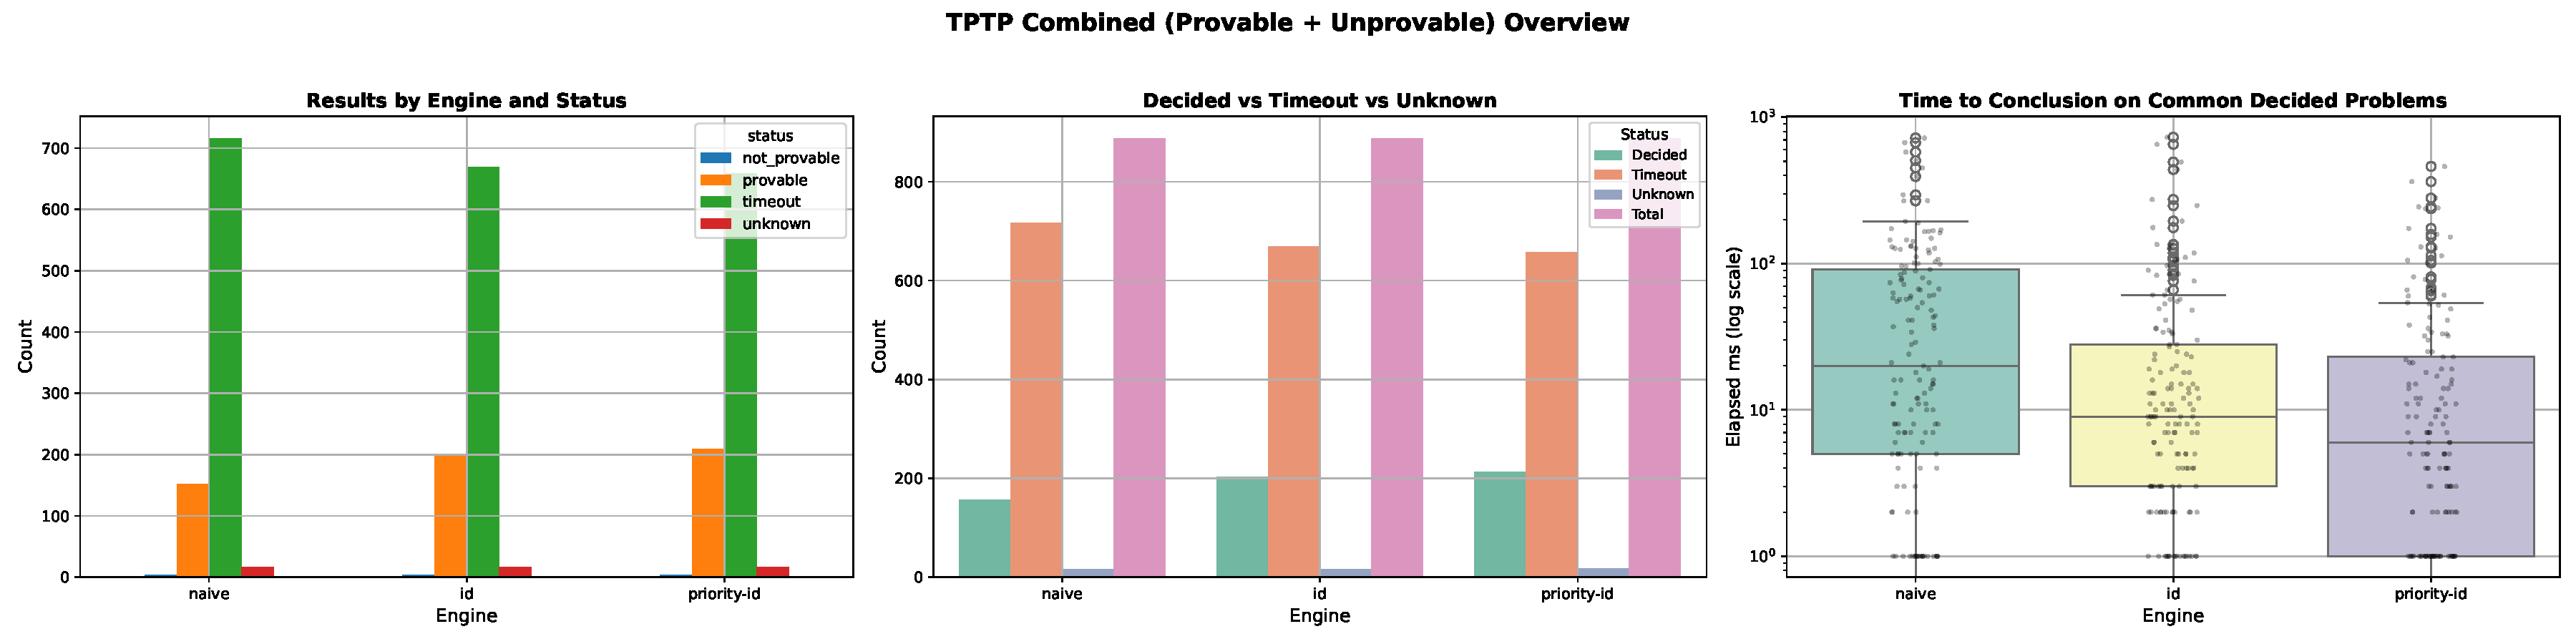
\includegraphics[width=\linewidth]{figures/tptp_combined_overview.pdf}
  \caption{TPTP combined dataset (888 problems): outcome counts by engine
    (left), decided vs.\ timeout vs.\ unknown breakdown (centre), and
  time to conclusion on commonly decided problems, log scale (right).}
  \label{fig:tptp-overview}
\end{figure}

\begin{figure}[h]
  \centering
  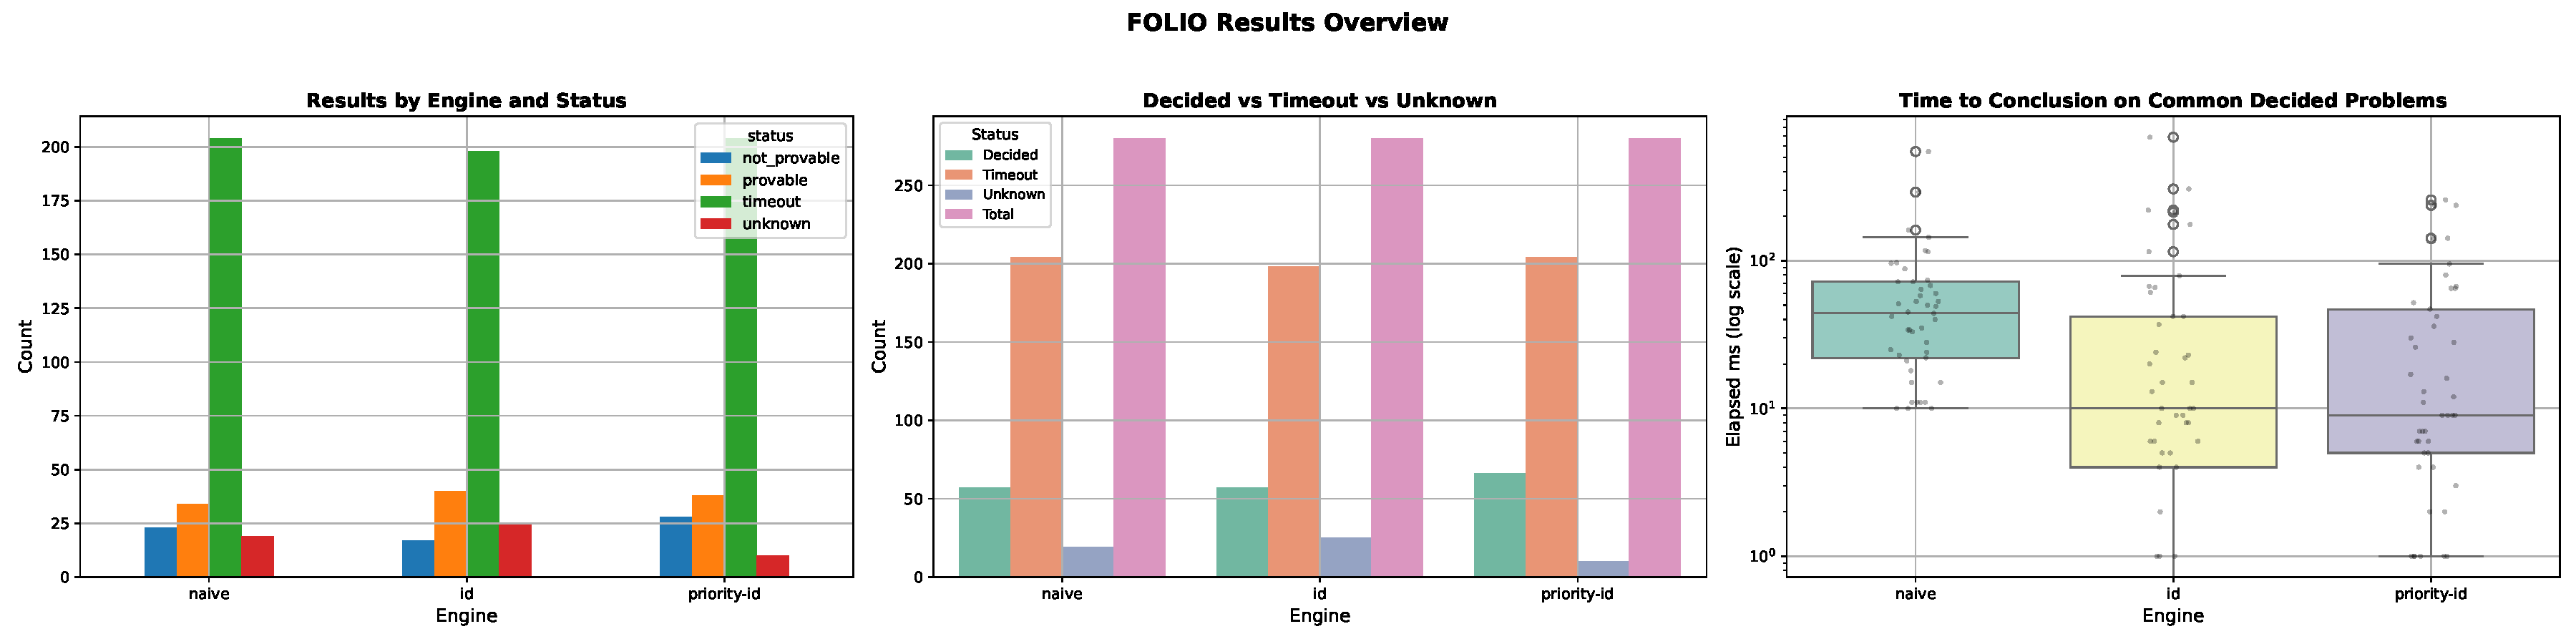
\includegraphics[width=\linewidth]{figures/folio_overview.pdf}
  \caption{FOLIO validation set (280 problems): outcome counts by engine
    (left), decided vs.\ timeout vs.\ unknown breakdown (centre), and
  time to conclusion on commonly decided problems, log scale (right).}
  \label{fig:folio-overview}
\end{figure}

\begin{figure}[h]
  \centering
  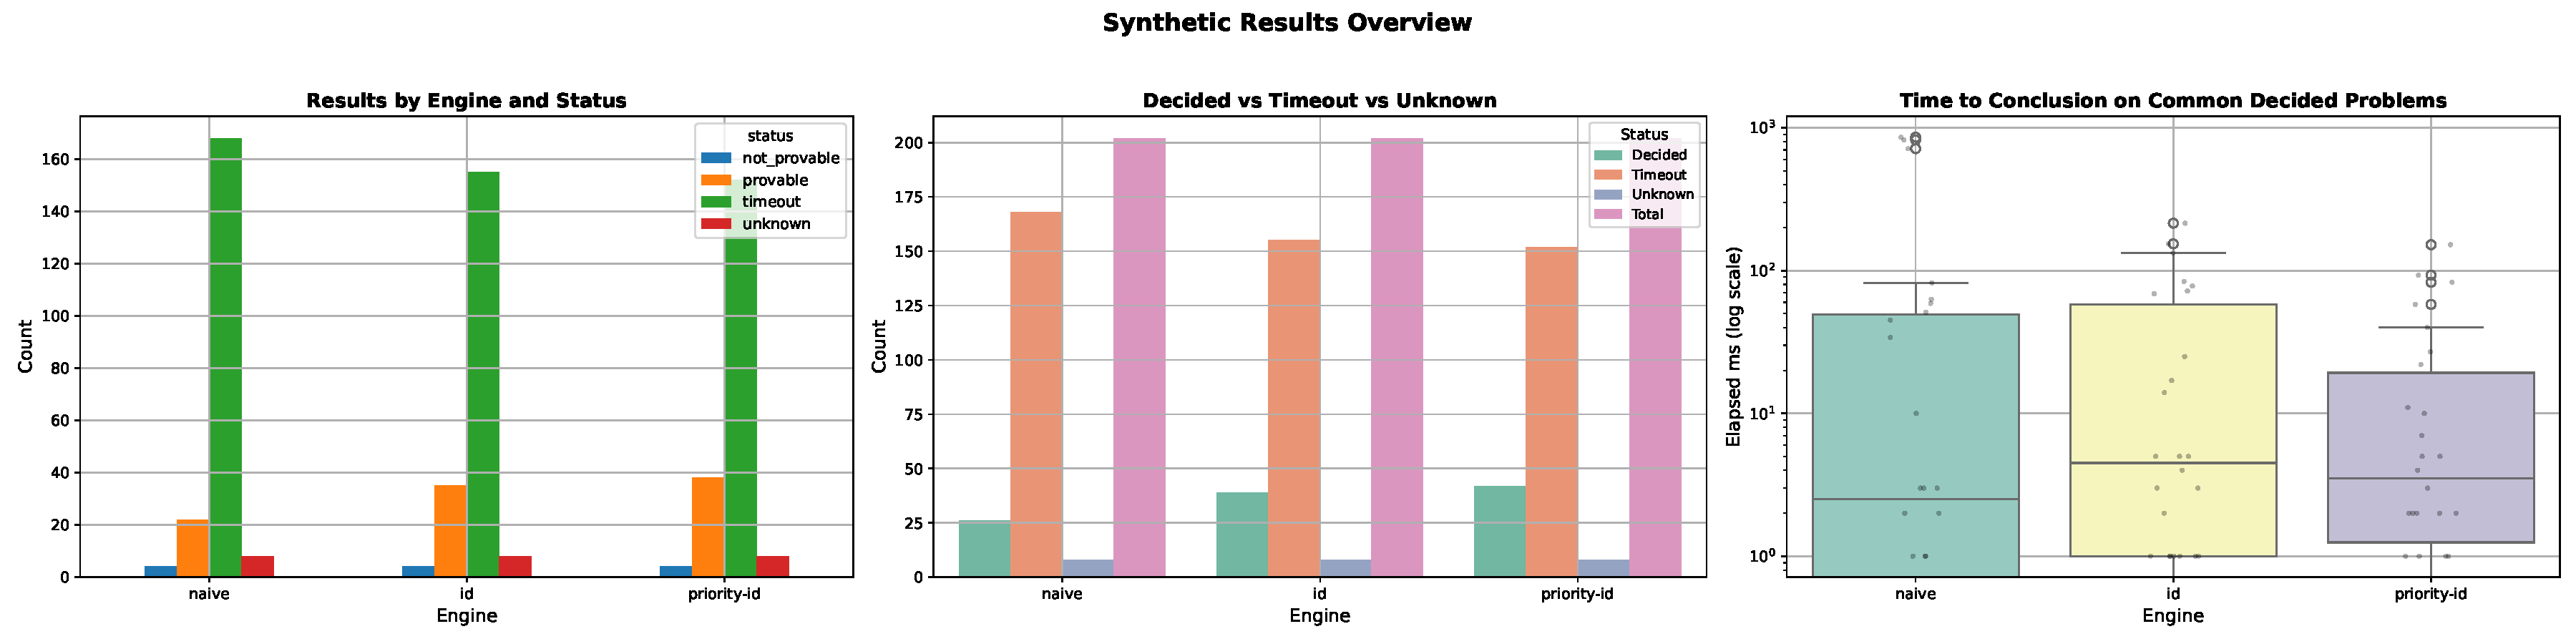
\includegraphics[width=\linewidth]{figures/generated_overview.pdf}
  \caption{Synthetic dataset (202 problems): outcome counts by engine
    (left), decided vs.\ timeout vs.\ unknown breakdown (centre), and
  time to conclusion on commonly decided problems, log scale (right).}
  \label{fig:ai-overview}
\end{figure}

\begin{figure}[h]
  \centering
  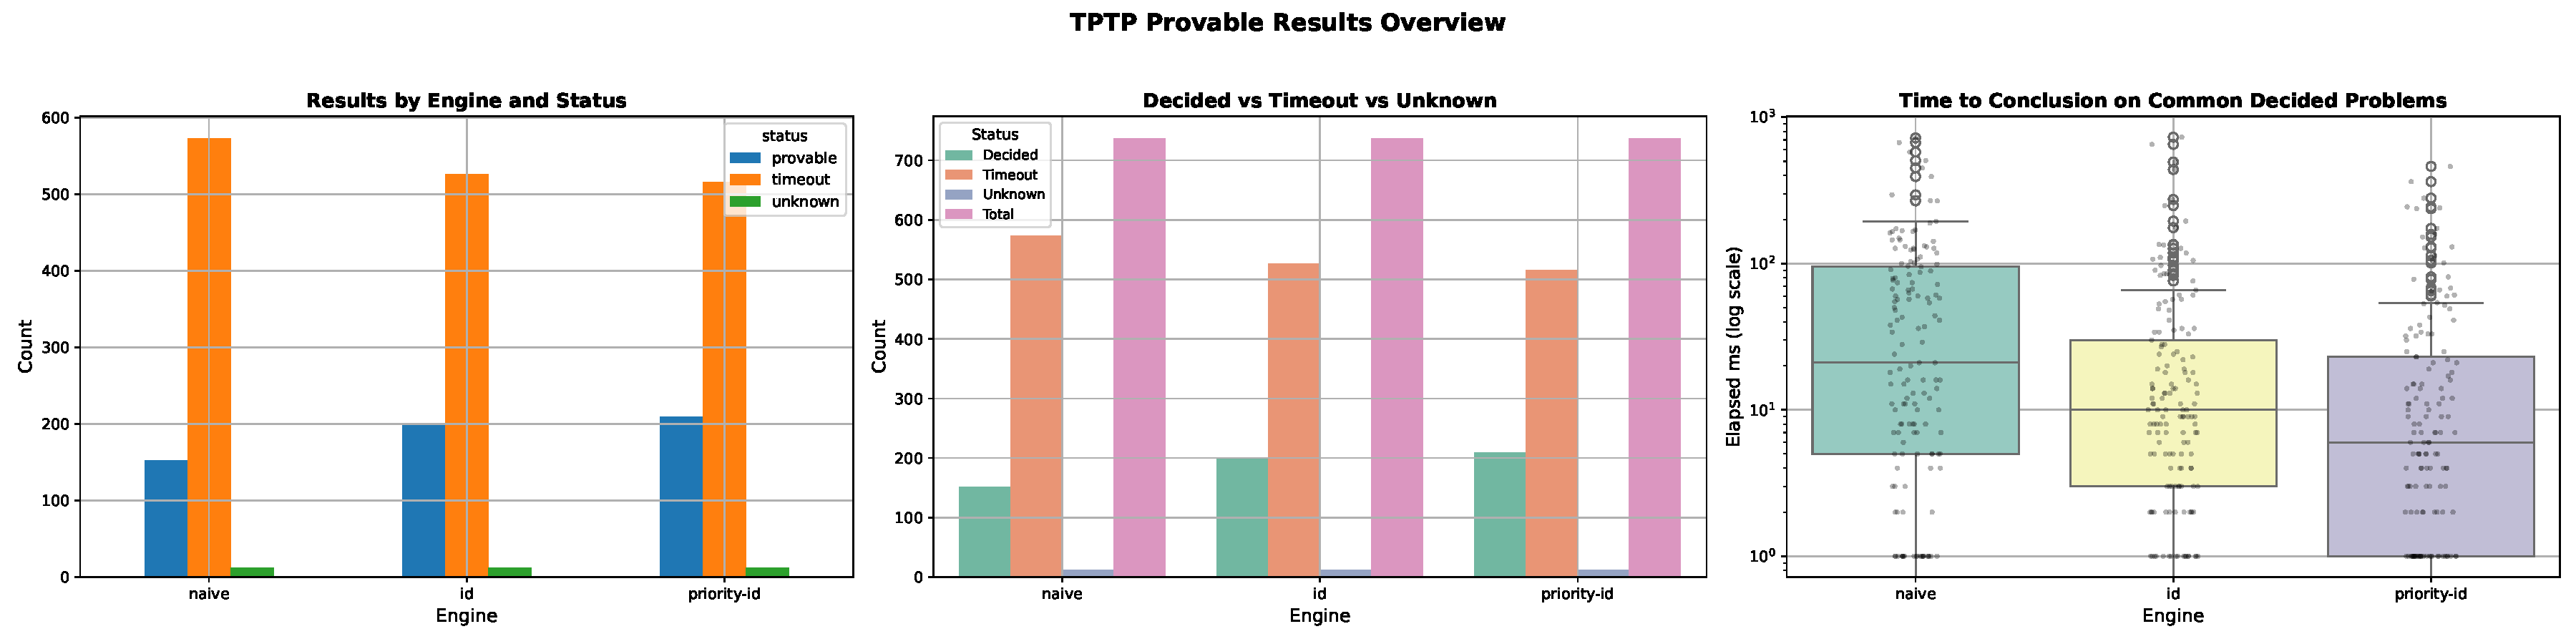
\includegraphics[width=\linewidth]{figures/tptp_provable_overview.pdf}
  \caption{TPTP provable subset (737 problems): outcome counts by engine,
    decided vs.\ timeout vs.\ unknown, and timing. See
  Table~\ref{tab:tptp-provable} for numerical breakdown.}
  \label{fig:tptp-provable}
\end{figure}

\begin{figure}[h]
  \centering
  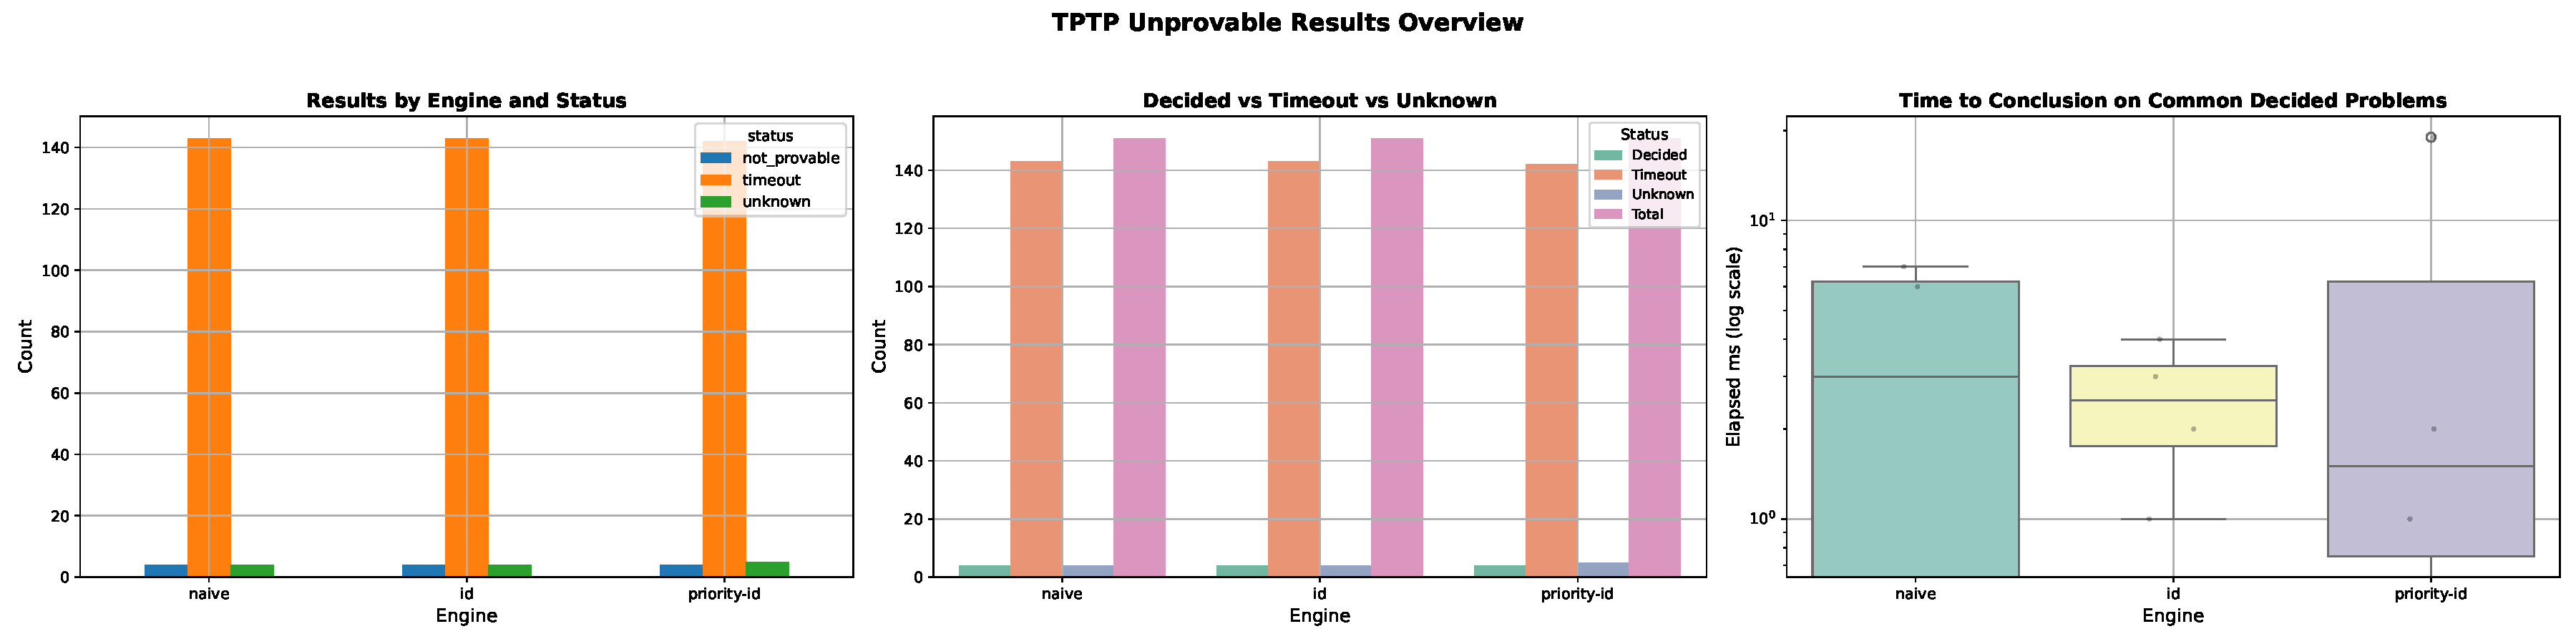
\includegraphics[width=\linewidth]{figures/tptp_unprovable_overview.pdf}
  \caption{TPTP counter-satisfiable subset (151 problems): outcome counts by
    engine, decided vs.\ timeout vs.\ unknown, and timing. See
  Table~\ref{tab:tptp-unprovable} for numerical breakdown.}
  \label{fig:tptp-unprovable}
\end{figure}

\begin{figure}[h]
  \centering
  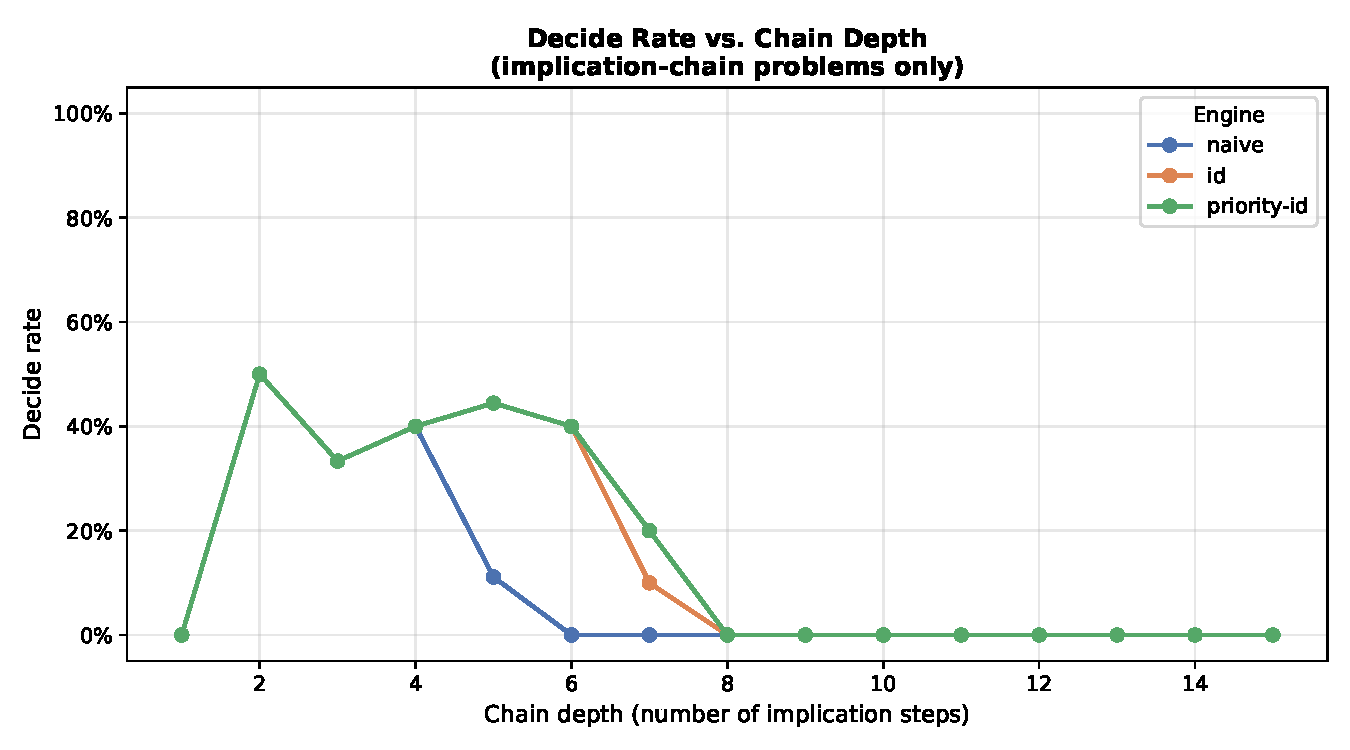
\includegraphics[width=0.85\linewidth]{figures/generated_depth_decide_rate.pdf}
  \caption{Decision rate vs.\ chain depth for implication-chain problems
  (fraction decided per depth, by engine).}
  \label{fig:synthetic-depth}
\end{figure}

\begin{figure}[h]
  \centering
  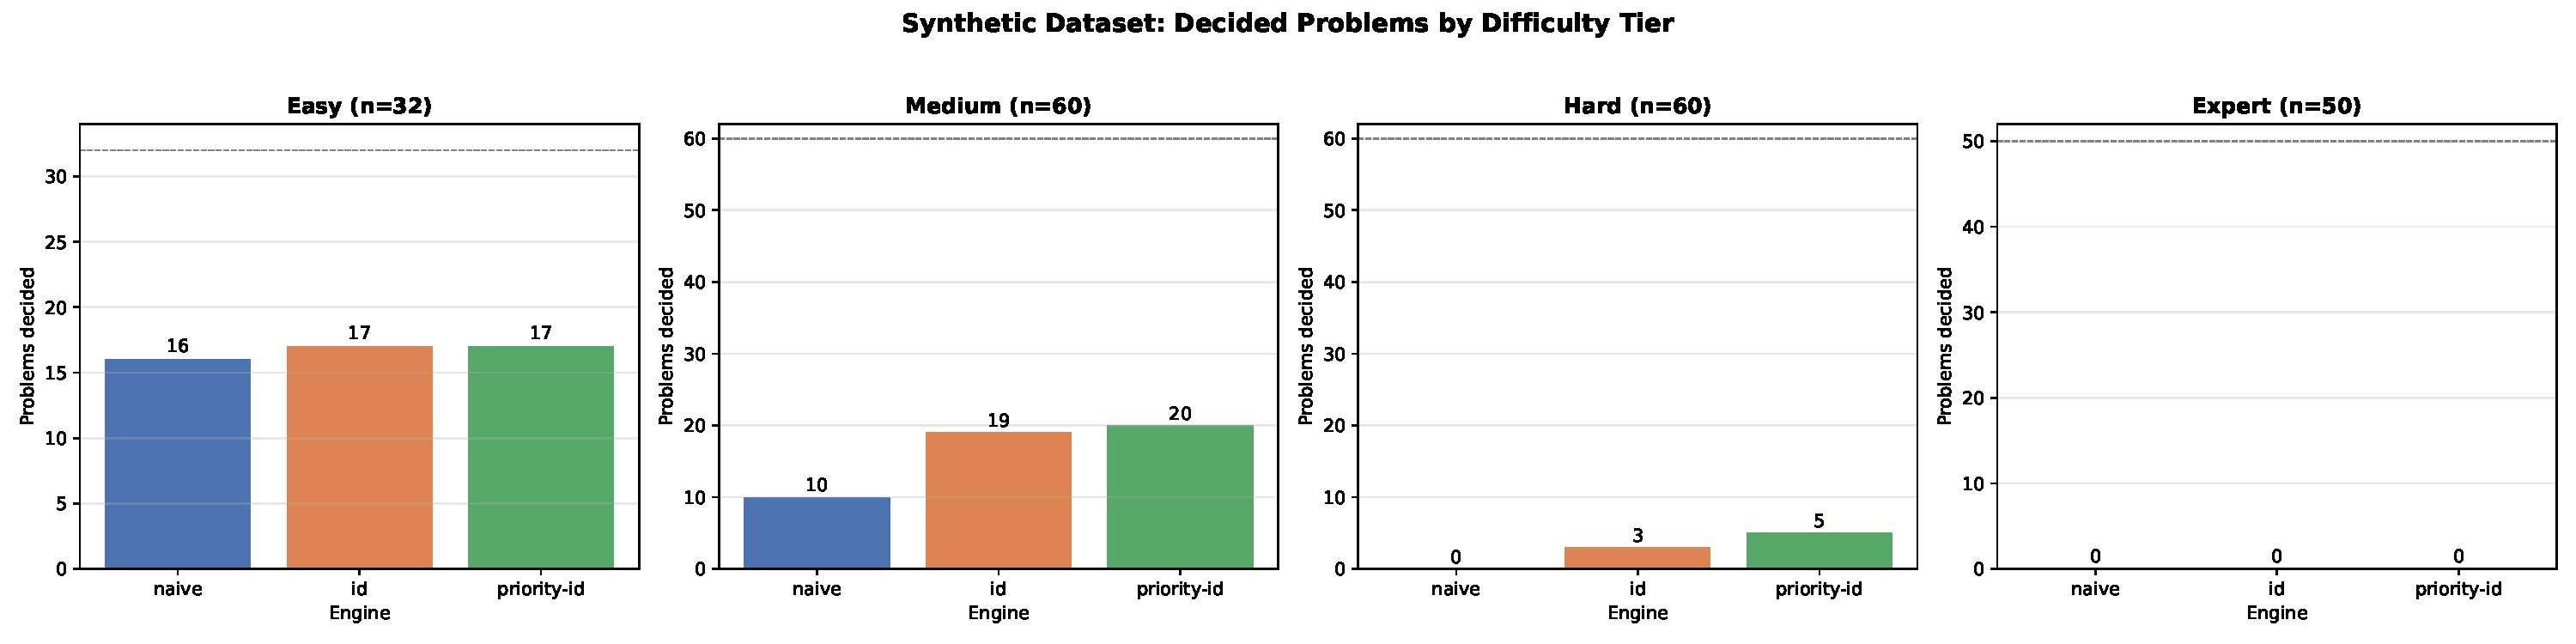
\includegraphics[width=\linewidth]{figures/generated_tier_breakdown.pdf}
  \caption{Synthetic dataset (202 problems): decided problems per engine
    at each difficulty tier. The dashed line marks the total number of
  problems in that tier.}
  \label{fig:synthetic-tier}
\end{figure}

\begin{figure}[h]
  \centering
  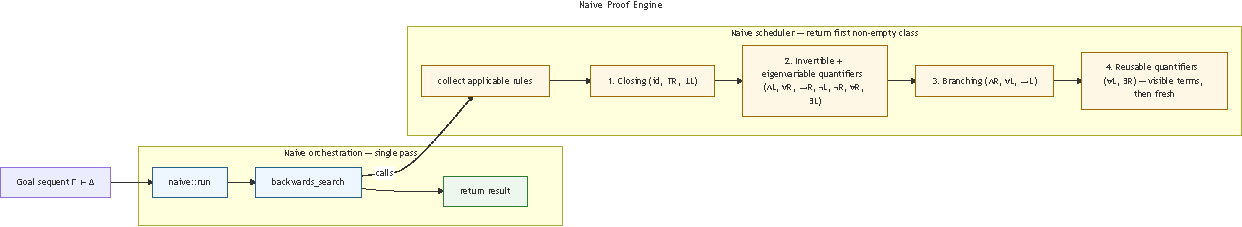
\includegraphics[width=\linewidth]{figures/naive_engine_diagram.pdf}
  \caption{Naive proof engine: single-pass DFS with the five-group
  naive scheduler.}
  \label{fig:naive-engine}
\end{figure}

\FloatBarrier
\section{Generative AI Use}\label{app:ai}

Two AI tools were used heavily for code development. Where possible,
queries are reproduced from session logs with minor typographical corrections
for readability but are otherwise verbatim; those corrections were themselves
made with Claude Sonnet 4.6 assistance.

\textbf{Claude Sonnet~4.6} (Anthropic), accessed via the Claude Code
command-line interface and web interface (\texttt{claude.ai/code}), was the
primary tool. All Claude-assisted commits carry a
\texttt{Co-Authored-By: Claude Sonnet~4.6} trailer that Claude Code
automatically appends, providing verifiable attribution in the git history.
The following queries and responses are reproduced from local Claude Code
session logs (\texttt{.jsonl} files stored by the CLI); the
priority-scheduler session (\S\ref{app:ai-scheduler}) was conducted via the
web interface and is documented from commit trailers only, as no local log
was retained.

\textbf{OpenAI Codex} was also used during development for feature
implementation, design discussion, and code-quality passes. Session logs were
not retained for Codex interactions and Codex does not automatically tag
commits, so specific queries cannot be reproduced.

\subsection*{A.2.1\quad Iterative Deepening Engine (6 May 2026)}

\textbf{Queries:}
\begin{quote}
  I want to implement an iterative deepening backwards search engine. The
  feature may not need to be a full engine, but the idea is to use the clap CLI
  args so the user can select via \texttt{--engine naive} or
  \texttt{--engine id}.
  I will be adding more optimisations later, but this is the starting point. The
  current architecture should support iterative deepening. Here is
  the algorithm:
  [Algorithm~2, p.~67, Hou 2021, supplied as full \LaTeX\ pseudocode].
\end{quote}

\begin{quote}
  I started an ultraplan session in the web browser and it began editing code.
  I would like to continue from the CLI instead, using this plan:
  [Plan: Iterative Deepening Backward Search Engine --- \texttt{--engine} flag,
    \texttt{ProofOptions::engine} field, ID loop calling
    \texttt{backwards\_search}
  at increasing depth limits, \texttt{engine/id.rs} module].
\end{quote}

\begin{quote}
  Please also make sure the engine can be configured in \texttt{config.toml},
  that everything is documented appropriately, and that all relevant functions
  have appropriate rustdocs.
\end{quote}

\textbf{Outcome:} Claude implemented the \texttt{--engine naive|id} CLI flag,
\texttt{ProofOptions::engine} field, and the iterative-deepening loop in a new
\texttt{engine/id.rs} submodule, adding rustdocs throughout
(commits \texttt{d16bb3c} and associated engine-modularisation commits).

\subsection*{A.2.2\quad SQLite Persistence (6 May 2026)}

\textbf{Queries:}
\begin{quote}
  I need to make the results from each run for each engine persist so I can
  analyse the data. How should I do this?
\end{quote}

\begin{quote}
  SQLite would be preferable --- can we use that instead?
\end{quote}

\begin{quote}
  The interface should be something like \texttt{--persist true} or
  \texttt{--persist false}, defaulting to \texttt{true}, with the database
  location configurable --- perhaps \texttt{--persist <DB\_FILE\_LOCATION>} with
  a default path specified in \texttt{config.toml}.
\end{quote}

\begin{quote}
  The CLI flag wiring should live in \texttt{cli/}, but the actual insertion
  logic should be in its own module such as \texttt{src/persistence}.
  What is your recommendation?
\end{quote}

\textbf{Outcome:} Claude designed and implemented the \texttt{src/persistence/}
module with an SQLite schema, \texttt{--persist} CLI flag with configurable
path, and a TDD test suite (commits \texttt{a8333b8}, \texttt{c5bc21f},
\texttt{5719e21}, \texttt{ba06ddf}, \texttt{2ca6f0e}, \texttt{a1de674}).

\subsection*{A.2.3\quad Six-Class Priority Scheduler (6 May
2026)}\label{app:ai-scheduler}

\textbf{Note:} This session was conducted via the Claude Code web interface;
no local session log is available. The session is documented from the
\texttt{Co-Authored-By: Claude Sonnet 4.6 <noreply@anthropic.com>} trailers
that Claude Code automatically appends to commits it helps author.

\textbf{Outcome:} Claude implemented the six-class LK$'$ rule priority scheduler
(closing rules; non-branching propositional; branching propositional;
  eigenvariable quantifiers; reusable quantifiers with visible witnesses;
reusable quantifiers with fresh fallback) and the \texttt{Priority} and
\texttt{PriorityId} engine variants
(commits \texttt{8d72635}, \texttt{663ac9a}, \texttt{d16bb3c}).

\subsection*{A.2.4\quad FOLIO Rust Integration (9 May 2026)}

\textbf{Queries:}
\begin{quote}
  I am happy to modify the prover so that it does not require a \texttt{.p}
  file --- it can be adapted to accept whatever format is needed.
  Please have a look at \texttt{theorem\_prover/} to determine the
  best approach.
\end{quote}

\begin{quote}
  Ensure every new function is appropriately documented with rustdocs, and
  maintain appropriate separation of concerns across modules, files, and
  functions. Create new submodules or files where needed to meet good software
  design standards.
\end{quote}

\textbf{Outcome:} Claude extended the grammar and parser to accept FOLIO
\texttt{.jsonl} problems directly without converting to TPTP \texttt{.p}
format, adding a new parser module with full rustdoc coverage.

\subsection*{A.2.5\quad Parallelisation and Channel-Based DB Writer
(9 May 2026)}

\textbf{Queries:}
\begin{quote}
  I would like to run problem files in parallel within
  \texttt{theorem\_prover/}.
  I am considering migrating persistence from SQLite to PostgreSQL to support
  this, though I am not sure that is the right approach.
\end{quote}

\begin{quote}
  For parallelisation: multiple files simultaneously within a single invocation.
\end{quote}

\begin{quote}
  Out-of-order progress output is acceptable. Please implement this with TDD.
  The timer logic can also be simplified, and the Ctrl-C handling can likely be
  simplified now that the owner thread can terminate the workers directly.
\end{quote}

\textbf{Outcome:} Claude implemented \texttt{rayon} \texttt{par\_iter} over
problem paths with an \texttt{AtomicUsize} progress counter, a channel-based
SQLite writer thread to avoid connection-sharing across threads, and an
exit-code fix (\texttt{process::exit} replaced with a return value to ensure
the writer thread flushes before exit)
(commits \texttt{c52a7bf}, \texttt{95cc45a}, \texttt{d48cc7b}).

